\icode{E-MD-CA-L2-261114-006}
如图一可视为质点的物体，在倾角 $\theta = $\,\qty{30}{\degree} 的固定斜面上，向下轻轻一推，它恰好匀速下滑。已知斜面长度为 $L = $\,\qty{5}{m}。求：欲使物体由斜面底端开始，沿斜面冲到顶端，物体上滑时的初速度至少为多大？（\(g\)取\qty{10}{m/s^2}）

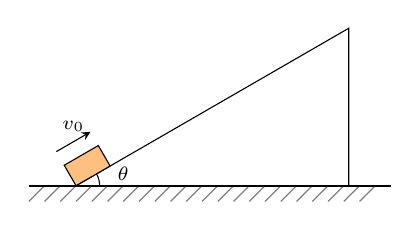
\begin{tikzpicture}[>=stealth,font=\scriptsize]
	\begin{scope}[rotate=30]
		\draw (0,0)--(0:4)--++(-120:2);
		\draw[fill=orange!50] (0,0) rectangle(.5,.3);
		\draw[->] (0,.5)--node[above]{\(v_0\)}(.5,.5);
	\end{scope}
	\draw (.3,0) arc(0:30:.3);
	\node at(.6,.15){\(\theta\)};
	\foreach \x in {-.6,-.4,...,3.8}
		\draw[gray] (\x,-.2)--++(.2,.2);
	\draw[thick] (-.6,0)--(4,0);
\end{tikzpicture}
\begin{answer}
    \qty{10}{m/s}
\end{answer}